\documentclass{beamer}

\usepackage{amsmath}
\usepackage{amsthm}
\usepackage{amsfonts}
\usepackage{amssymb}
\usepackage{times}
\usepackage{verbatim}
\usepackage{multirow}
\usepackage{xspace}
\usepackage{contour}


\definecolor{pbdgrn}{HTML}{005700}
\definecolor{pbdrd}{HTML}{ab0000}
\definecolor{pbdylw}{HTML}{ab7e00}
\definecolor{pbdblu}{HTML}{2b74ec}

\contourlength{0.5pt} %how thick each copy is
\contournumber{5}  %number of copies
\newcommand{\pbdR}{%
%   \textbf{
%     \color{pbdgrn}p\color{pbdrd}b\color{pbdylw}d\color{pbdblu}R}
%   }
\contour{black}{\protect\textcolor{pbdgrn}{p}}%
\contour{black}{\protect\textcolor{pbdrd}{b}}%
\contour{black}{\protect\textcolor{pbdylw}{d}}%
\contour{black}{\protect\textcolor{pbdblu}{R}}\xspace
}

\newcommand{\R}{%
  \textsf{R}
}


\definecolor{myblack}{rgb}{0,0,0}
\definecolor{mygreen}{rgb}{0,0.5,0}
\definecolor{mygreen3}{rgb}{0,0.69,0.09}
\definecolor{myred}{rgb}{1,0,0}
\definecolor{myblue3}{rgb}{0,0,0.8}
\definecolor{mymagenta3}{rgb}{0.8,0,0.8}
\definecolor{mydarkred}{rgb}{0.5,0,0}
\definecolor{dgreen}{rgb}{0.0,0.52,0.27}

\newcommand{\colorA}{\mbox{\color{mygreen3} A}}
\newcommand{\colorC}{\mbox{\color{mymagenta3} C}}
\newcommand{\colorG}{\mbox{\color{myblue3} G}}
\newcommand{\colorT}{\mbox{\color{myred} T}}
\newcommand{\colorcdots}{\color{myblack} $\cdots$}

\newcommand{\vect}[1]{\boldsymbol{#1}}
\newcommand{\argmax}{\operatornamewithlimits{argmax}}
\newcommand{\dmax}[1]{{\displaystyle \max_{#1}\;}}
\newcommand{\dargmax}[1]{{\displaystyle \argmax_{#1}\;}}

\newcommand{\A}{\mbox{A}}
\newcommand{\C}{\mbox{C}}
\newcommand{\G}{\mbox{G}}
\newcommand{\T}{\mbox{T}}
\newcommand{\piA}{\pi_{\mbox{\tiny \colorA}}}
\newcommand{\piC}{\pi_{\mbox{\tiny \colorC}}}
\newcommand{\piG}{\pi_{\mbox{\tiny \colorG}}}
\newcommand{\piT}{\pi_{\mbox{\tiny \colorT}}}
\newcommand{\deltaAG}{\delta_{\mbox{\tiny A}\mbox{\tiny G}}}
\newcommand{\deltaCT}{\delta_{\mbox{\tiny C}\mbox{\tiny T}}}
\newcommand{\DeltaAGCT}{\Delta^{\mbox{\tiny A}\mbox{\tiny G}}_{\mbox{\tiny C}\mbox{\tiny T}}}
\newcommand{\DeltaCTAG}{\Delta^{\mbox{\tiny C}\mbox{\tiny T}}_{\mbox{\tiny A}\mbox{\tiny G}}}

\newcommand{\E}{\mathbb{E}}


%
% Choose how your presentation looks.
%
% For more themes, color themes and font themes, see:
% http://deic.uab.es/~iblanes/beamer_gallery/index_by_theme.html
%
\mode<presentation>
{
  \usetheme{default}      % or try Darmstadt, Madrid, Warsaw, ...
  \usecolortheme{default} % or try albatross, beaver, crane, ...
  \usefonttheme{default}  % or try serif, structurebold, ...
  \setbeamertemplate{navigation symbols}{}
  \setbeamertemplate{caption}[numbered]
  \setbeamertemplate{footline}[frame number]
} 

\usepackage[english]{babel}


\title[Phyloclustering]{Phyloclustering: A Model-Based Approach for Identifying Microbial Populations}
\author{\large Wei-Chen Chen}
\institute{\normalsize \pbdR Core Team}
\date{\small 2018 Symposium on Data Science and Statistics (SDSS)}

\begin{document}

\begin{frame}
  \titlepage
\end{frame}

\begin{frame}{Disclaimer}
Any opinions, findings, and conclusions or recommendations expressed in
this presentation are those of the authors.

\vspace{\baselineskip}

Nothing in this content has been formally disseminated by the U.S. Department
of Health \& Human Services or by U.S. Food and Drug Administration,
and should not be construed to represent any determination
or policy of University, Agency, Administration, or National Laboratory.
\end{frame}

%-----------------------------------------------------------------------------

% Uncomment these lines for an automatically generated outline.
\begin{frame}{Outline}
  \tableofcontents
\end{frame}

%-----------------------------------------------------------------------------

\section{Motivation}
\subsection{Equine Infectious Anemia Virus (EIAV)}

\begin{frame}{Motivation I}
Equine Infectious Anemia Virus (EIAV)
\begin{itemize}
\item Leroux, Cador$\acute{\mbox{e}}$, and Montelaro (2004).
\item "Country cousin" of HIV.
\item Lentivirus in the Retrovirus family infect equines.
\item A persistent infection characterized by
      recurring febrile episodes associating with viremia,
      thrombocytopenia, and wasting symptoms.

\begin{columns}

\begin{column}{0.4\textwidth}
  \begin{figure}
  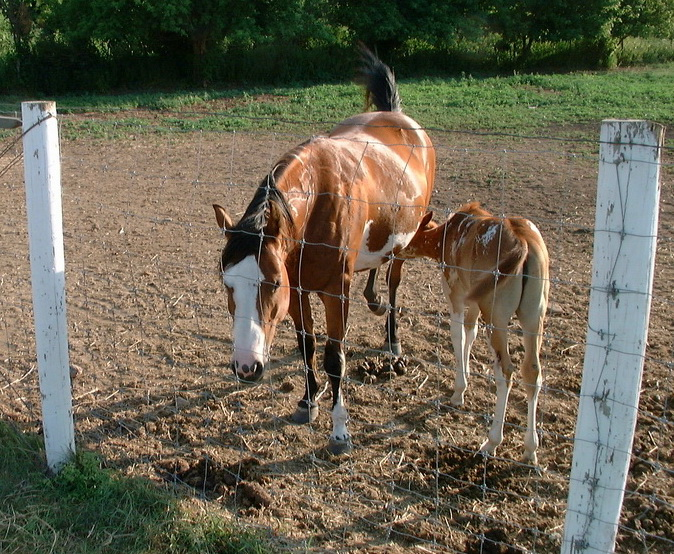
\includegraphics[width=\textwidth]{./graph/pony}
  \\
  {\tiny ISU Horse Barn (2006).}
  \end{figure}
\end{column}

\hspace{-0.2cm}

\begin{column}{0.7\textwidth}
  \begin{figure}
  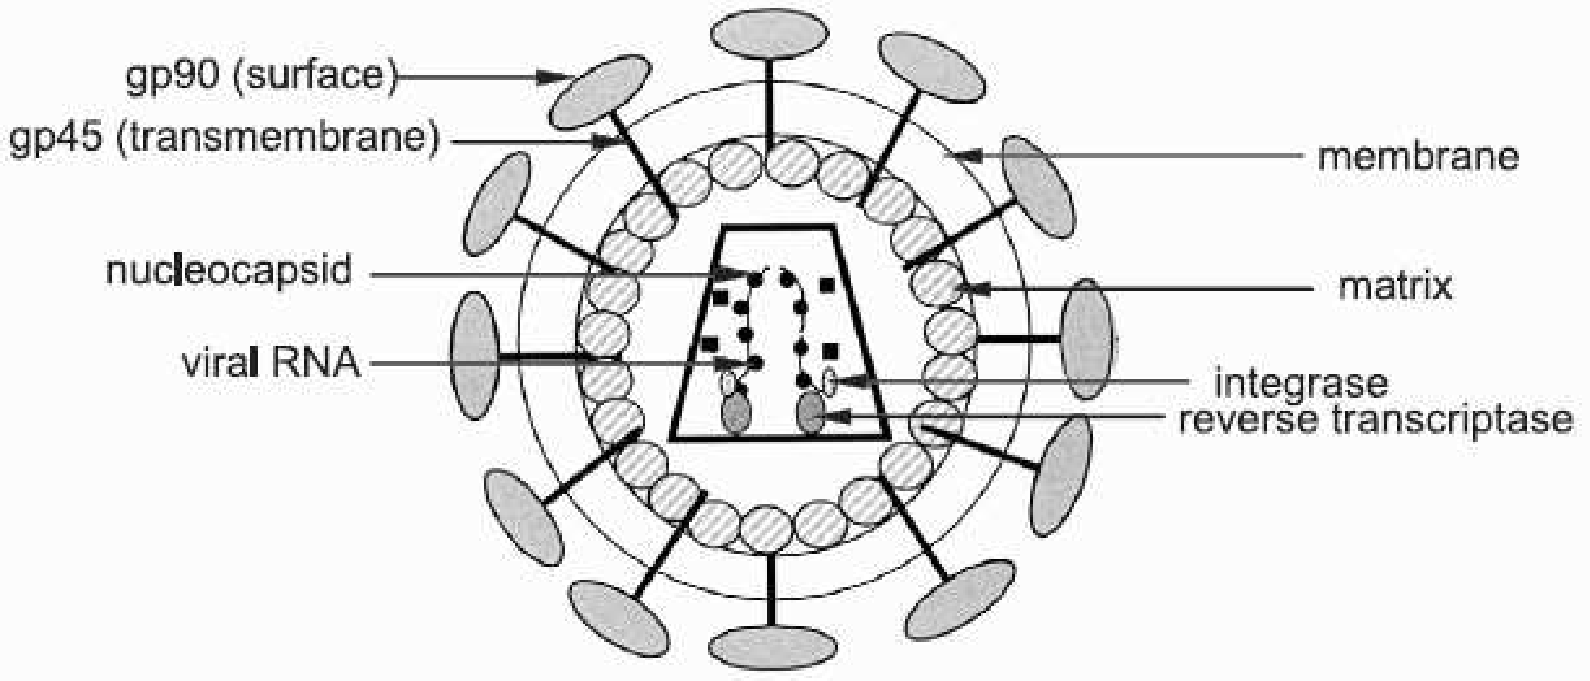
\includegraphics[width=\textwidth]{./graph/eiav_virus}
  \\
  {\tiny Leroux, Cador$\acute{\mbox{e}}$, and Montelaro (2004).}
  \end{figure}
\end{column}

\end{columns}

\end{itemize}
\end{frame}

%-----------------------------------------------------------------------------

\begin{frame}{Motivation II}
Phylogeny of Retroviruses
\vspace{-0.2cm}
\begin{figure}
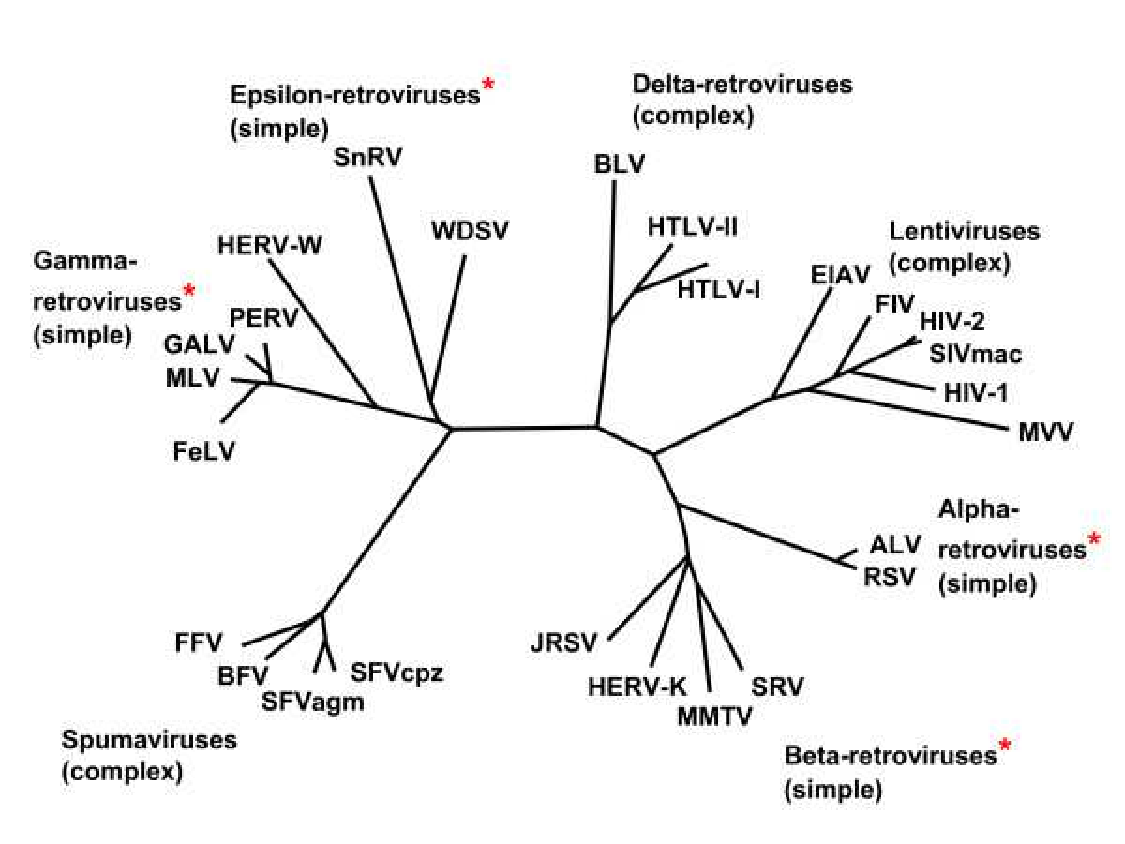
\includegraphics[width=0.9\textwidth]{./graph/retroviruses}
\\
{\tiny Weiss (2006).}
\end{figure}

\end{frame}

%-----------------------------------------------------------------------------

\begin{frame}{Motivation III}
PAQ: Partition Analysis of Quasispecies (Baccam et.al. (2001)).
\vspace{-0.2cm}
\begin{figure}
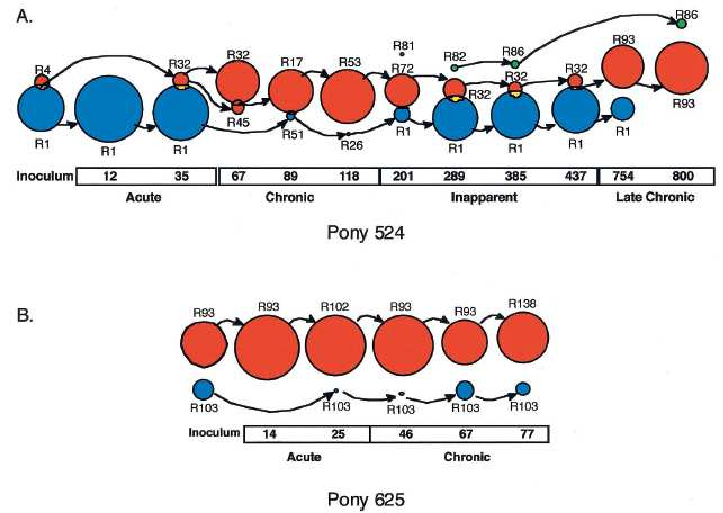
\includegraphics[width=0.9\textwidth]{./graph/paq}
\\
{\tiny Baccam et al. (2003).}
\end{figure}

\end{frame}

%-----------------------------------------------------------------------------

\begin{frame}{Motivation IV}
146 EIAV {\it rev} sequences of pony 524.

\vspace{-0.2cm}

\begin{columns}
\begin{column}{0.8\textwidth}
  \begin{figure}
  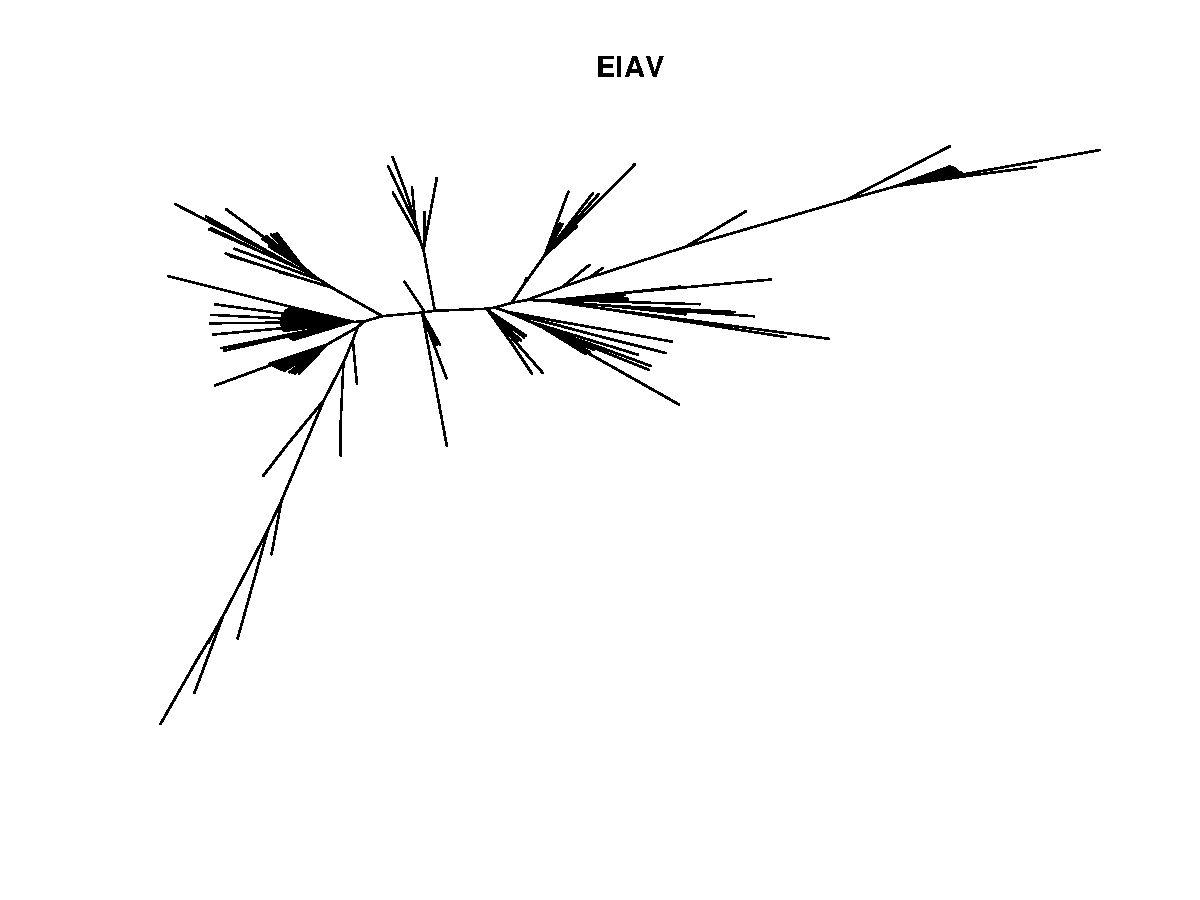
\includegraphics[width=\textwidth]{./graph/eiav_nj}
  \end{figure}
\end{column}

\hspace{-1.0cm}

\begin{column}{0.4\textwidth}
  \begin{figure}
  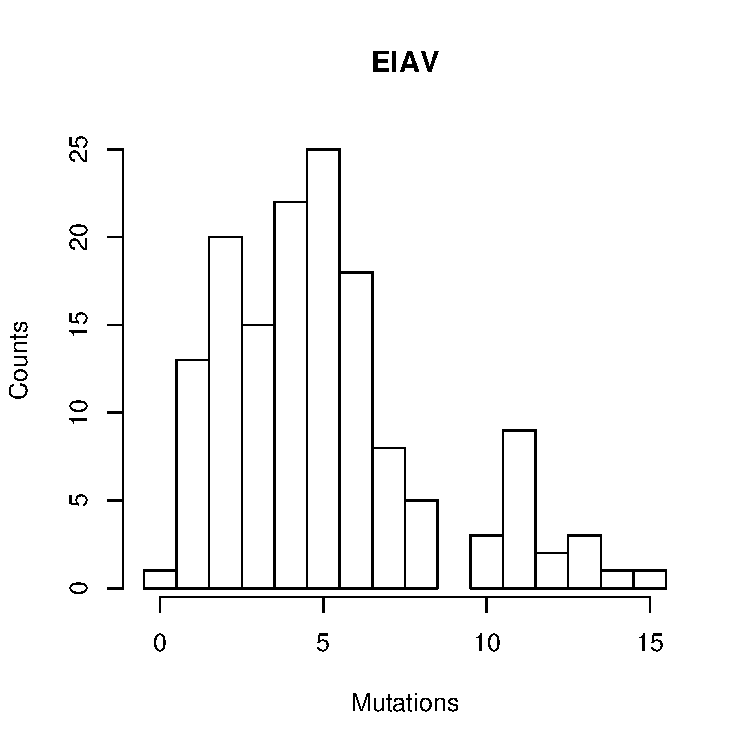
\includegraphics[width=\textwidth]{./graph/eiav_ht}
  \\
  {\tiny Mutation counts for 146 sequences.}
  %All pairwise difference average is 6.78 sites.}
  \end{figure}
\end{column}

\end{columns}

\end{frame}

%-----------------------------------------------------------------------------

\begin{frame}{Motivation V}
Number of bifurcating unrooted trees $N_U$ for $n\geq 3$ sequences is
$$
N_U = \frac{(2n - 5)!}{2^{n - 3} (n - 3)!}.
$$
\begin{center}
\begin{tabular}{cr} \hline\hline
Number of sequences & Number of unrooted trees \\ \hline
2 & 1 \\
3 & 1 \\
4 & 3 \\
5 & 15 \\
6 & 105 \\
7 & 945 \\
\vdots & \vdots \\
17 & 6,190,283,353,629,375 \\
18 & 191,898,783,962,510,625 \\
19 & 6,332,659,870,762,850,625 \\
20 & 221,643,095,476,699,771,875 \\ \hline\hline
\end{tabular}
\\
\scriptsize Felsenstein (1978) or Graur and Li (2000).
\end{center}

\end{frame}

%-----------------------------------------------------------------------------

\begin{frame}{Goals of Phyloclustering}
\begin{itemize}
\item to identify population centers where sequences may diverge from,
\item to establish a model based approach to cluster sequences
      with phylogenetic meaning,
\item to distinguish population structure based on classifications, and 
\item to aggregate trustworthy sequence information. 
\end{itemize}
\end{frame}

%-----------------------------------------------------------------------------

\section{Background}

\subsection{Mixture Multivariate Normal Distribution}

\begin{frame}{Mixture Multivariate Normal (MVN) Distribution}

Mixture MVN with $K$ components in $p$ dimension: \\
$X_1, \ldots, X_N \stackrel{iid}{\sim}
\phi(\vect{x} | \vect{\mu}, \vect{\Sigma})$
and
$
\phi(\vect{x}| \vect{\mu}, \vect{\Sigma})
= \sum_{k = 1}^K \eta_k \phi_k(\vect{x}| \vect{\mu}_k, \Sigma_k)
$
where
$
\phi_k(\vect{x} | \vect{\mu}_k, \vect{\Sigma}_k)
=
\frac{1}{(2\pi)^{p/2} |\Sigma_k|^{1/2}}
\exp\left\{-\frac{1}{2}
(\vect{x} - \vect{\mu}_k)^\prime \Sigma_k^{-1} (\vect{x} - \vect{\mu}_k)
\right\}
$

\vspace{-0.7cm}

\begin{columns}

\begin{column}{0.55\textwidth}
  \begin{figure}
  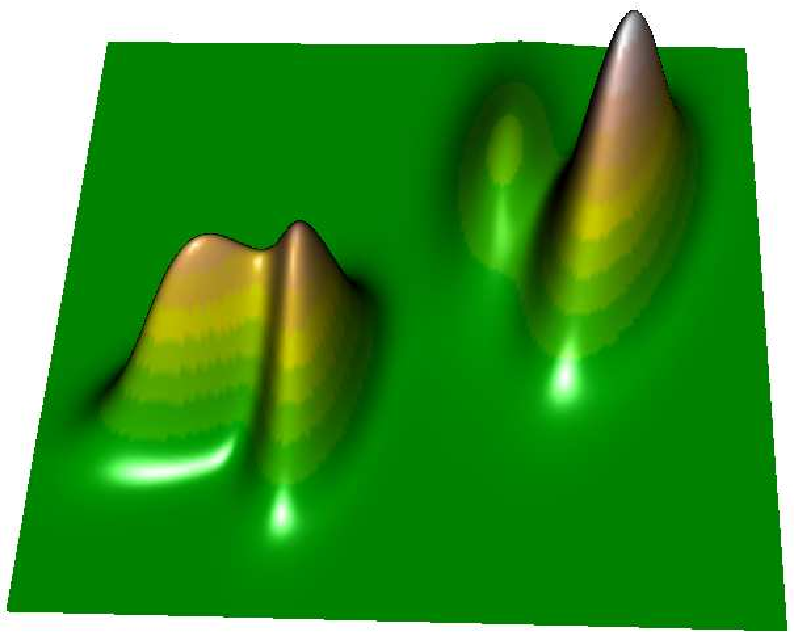
\includegraphics[width=\textwidth]{./graph/mixmvn_new}
  \end{figure}
\end{column}

\hspace{-0.3cm}

\begin{column}{0.55\textwidth}
  \begin{figure}
  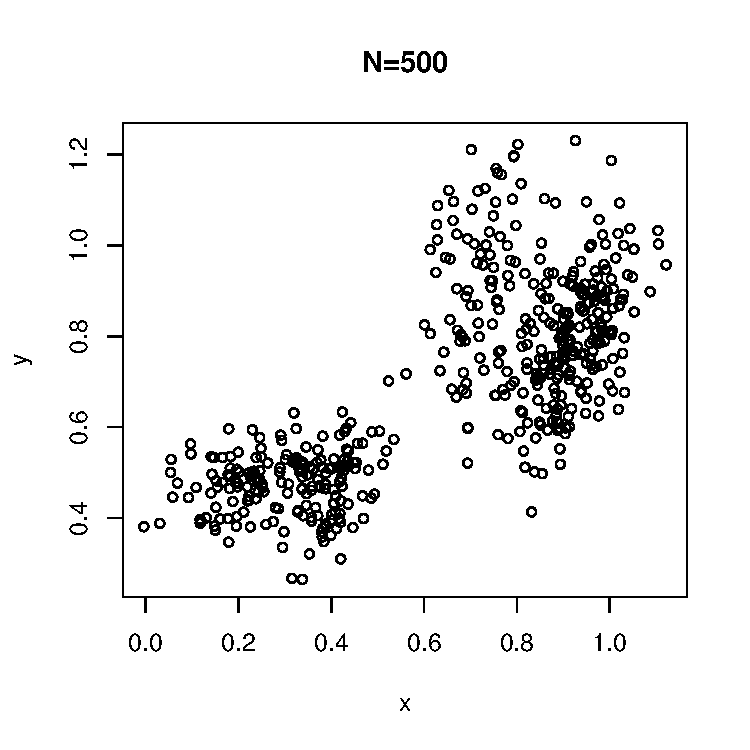
\includegraphics[width=\textwidth]{./graph/toy-1}
  \end{figure}
\end{column}

\end{columns}

\vspace{-0.2cm}

\begin{center}
\begin{color}{mydarkred}
Question: Are there four clusters? Where are they?
\end{color}
\end{center}

\end{frame}

%-----------------------------------------------------------------------------

\subsection{Model-based Clustering}

\begin{frame}{Model-based Clustering}
\vspace{-0.5cm}

\begin{figure}
  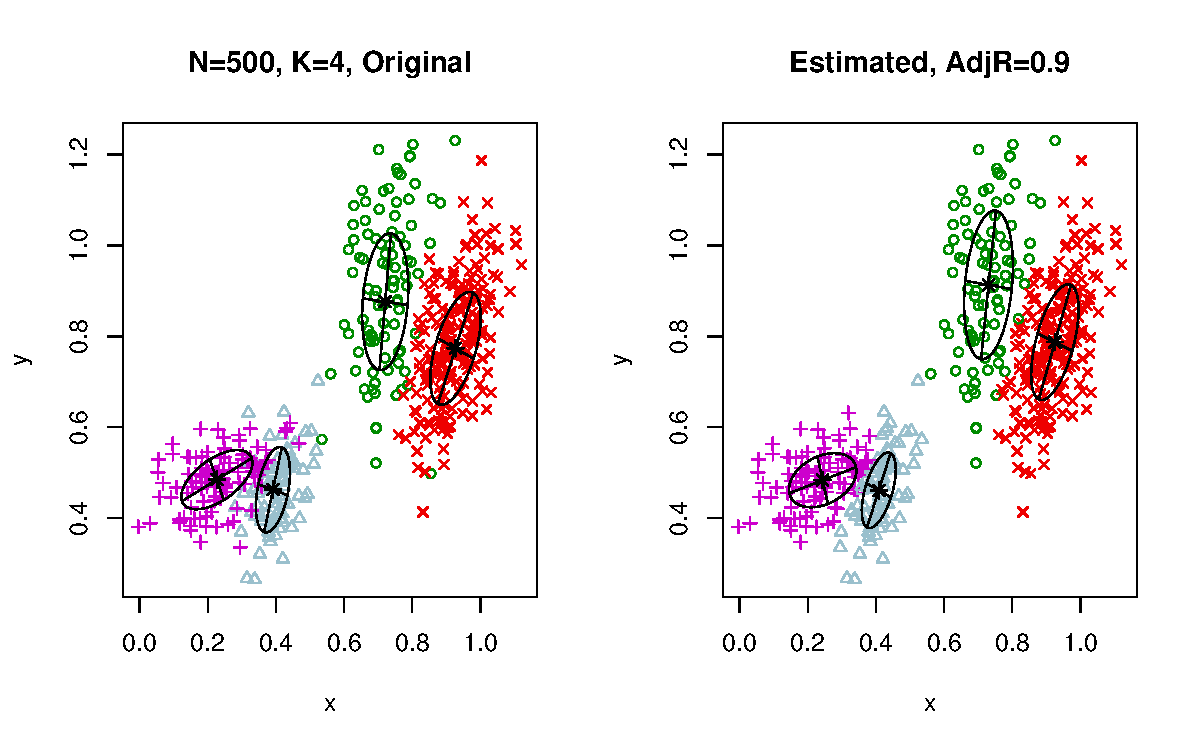
\includegraphics[width=\textwidth]{./graph/da4}
  \\
  {\tiny Model-based clustering based on the mixture MVN model.}
\end{figure}

\end{frame}

%-----------------------------------------------------------------------------

\subsection{Clustering for Nucleotide Sequences}

\begin{frame}{Clustering for Nucleotide Sequences}

\begin{columns}
\begin{column}{0.5\textwidth}
{\footnotesize
\begin{tabular}{cll} \hline\hline
Id & Sequence             & Center \\ \hline
1  & \colorA \colorC \colorG \colorT \colorC \colorG \colorT \colorC \colorcdots &
     \multirow{4}{*}{\colorA \colorA \colorG \colorT \colorC \colorG \colorT \colorG \colorcdots} \\
2  & \colorA \colorA \colorG \colorT \colorC \colorG \colorT \colorG \colorcdots & \\
3  & \colorA \colorA \colorG \colorT \colorC \colorG \colorA \colorG \colorcdots & \\
4  & \colorA \colorG \colorG \colorT \colorC \colorG \colorC \colorG \colorcdots & \\ \hline
5  & \colorC \colorC \colorG \colorG \colorA \colorC \colorA \colorC \colorcdots &
     \multirow{2}{*}{\colorC \colorC \colorG \colorG \colorA \colorC \colorA \colorC \colorcdots} \\
6  & \colorC \colorC \colorG \colorG \colorA \colorC \colorA \colorC \colorcdots & \\ \hline
7  & \colorC \colorT \colorT \colorG \colorC \colorC \colorG \colorC \colorcdots &
     \multirow{2}{*}{\colorC \colorT \colorT \colorT \colorC \colorC \colorG \colorC \colorcdots} \\
8  & \colorC \colorT \colorT \colorT \colorC \colorC \colorG \colorC \colorcdots & \\ \hline
9  & \colorA \colorG \colorG \colorT \colorC \colorC \colorT \colorC \colorcdots &
     \multirow{2}{*}{\colorA \colorG \colorG \colorT \colorC \colorC \colorT \colorC \colorcdots} \\
10 & \colorA \colorG \colorG \colorT \colorC \colorC \colorT \colorC \colorcdots & \\ \hline\hline
\end{tabular}
}
\end{column}

\begin{column}{0.5\textwidth}
\begin{figure}
  \vspace{-1.0cm}
  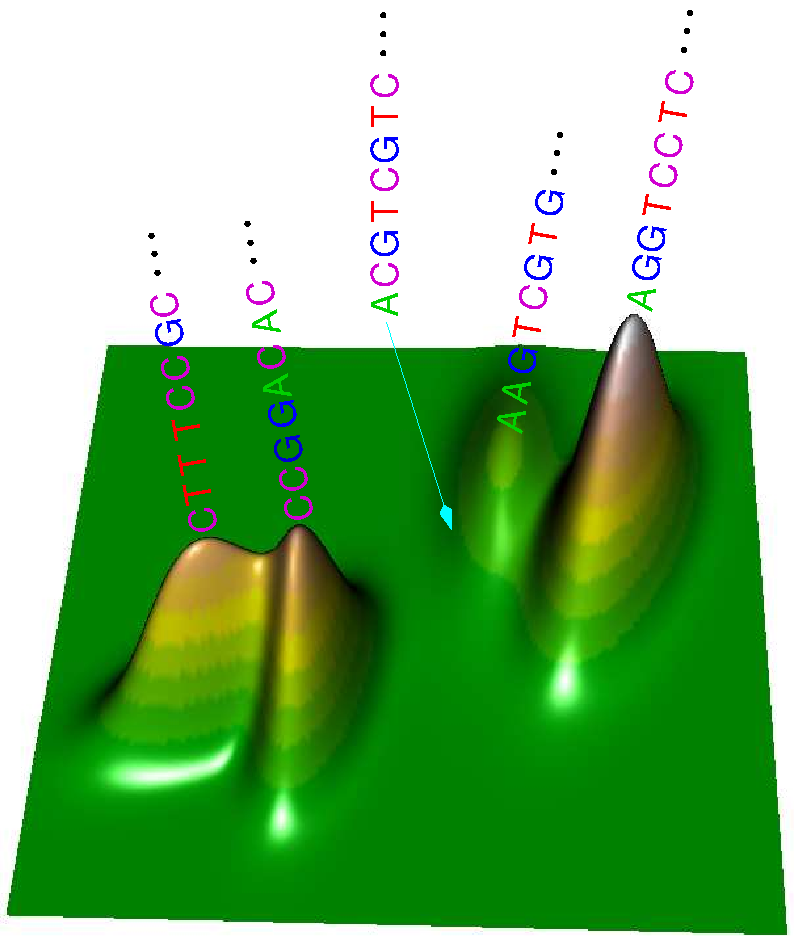
\includegraphics[width=\textwidth]{./graph/mixmvn_seq}
\end{figure}
\end{column}

\end{columns}

%\vspace{-0.5cm}
\begin{center}
\begin{color}{mydarkred}
Question: How do we model/cluster this kind of data?
\end{color}
\end{center}

\end{frame}

%-----------------------------------------------------------------------------

\begin{frame}{A Toy Dataset}

\vspace{-0.5cm}
\begin{figure}
  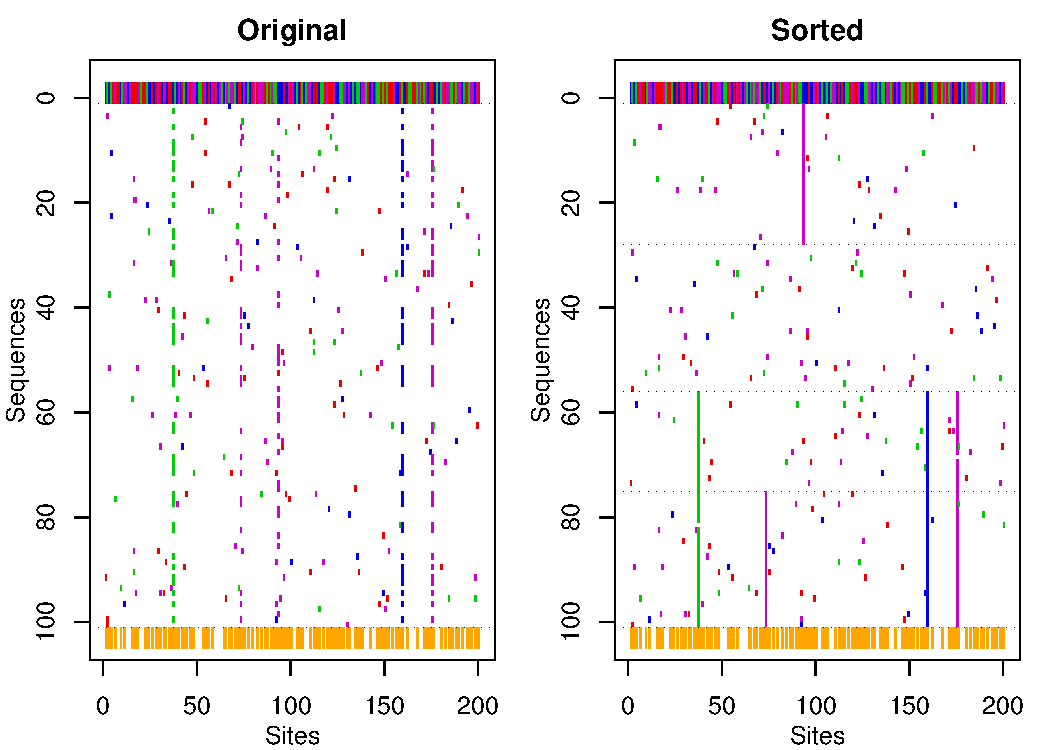
\includegraphics[width=4.3in]{./graph/seq-2_dot}
  \\
  {\tiny Green: \colorA, Blue: \colorG, Magenta: \colorC, Red: \colorT,
         Orange: segregating site.}
\end{figure}

\end{frame}

%-----------------------------------------------------------------------------

\begin{frame}{Phylogenetic Approach}

\vspace{0.5cm}
\begin{columns}

\begin{column}{0.5\textwidth}
  \begin{center}
  \small True tree for the toy dataset
  \vspace{-0.5cm}
  \begin{figure}
  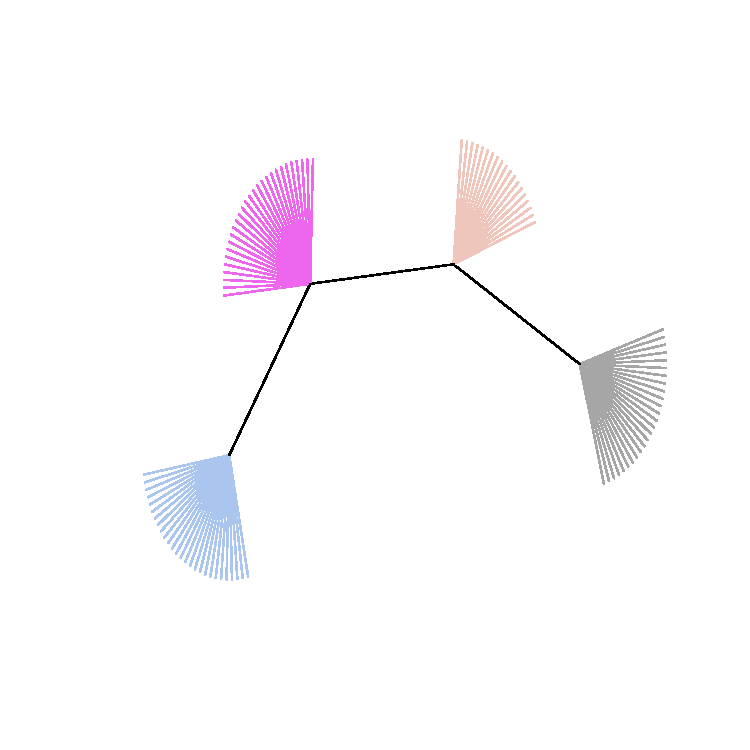
\includegraphics[width=1.05\textwidth]{./graph/seq-2_nj}
  \end{figure}
  \end{center}
\end{column}

\hspace{-0.5cm}

\begin{column}{0.5\textwidth}
  \begin{center}
  \small Neighbor joining tree (K80)
  \vspace{-0.5cm}
  \begin{figure}
  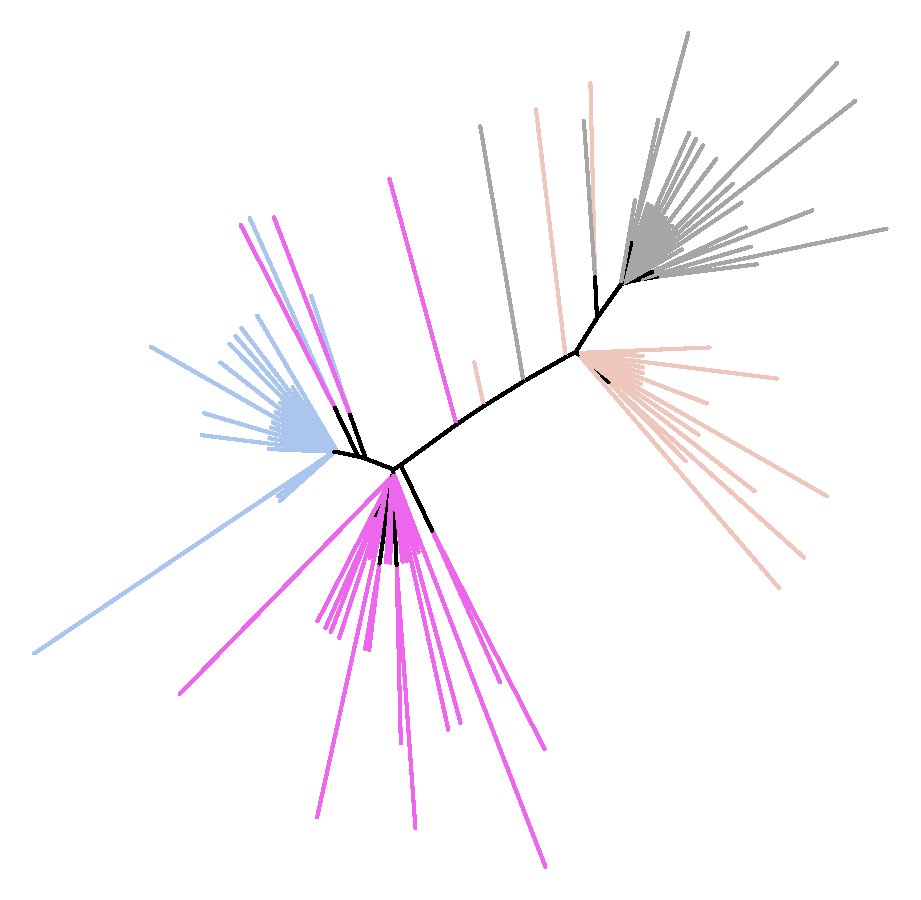
\includegraphics[width=1.05\textwidth]{./graph/seq-2_nj_K80}
  \end{figure}
  \end{center}
\end{column}

\end{columns}

\begin{center}
\color{mydarkred}
Question: What is the model for mutation process?
\end{center}

\end{frame}

%-----------------------------------------------------------------------------

\section{Phyloclustering Approach}

\subsection{Continuous Time Markov Chain (CTMC) Model}

\begin{frame}{Continuous Time Markov Chain (CTMC) Model}

\vspace{0.2cm}
Nucleotide substitution model: JC69
(Jukes \& Cantor (1969)), K80 (Kimura (1980)),
HKY85 (Hasegawa, Kishino \& Yano (1985)).
\\
\begin{columns}

\begin{column}{0.8\textwidth}
\hspace{0.1cm}
For example, HKY85 defines
$\vect{Q}_{x,y} = (q_{xy})_{4\times 4}$ as
\[
q_{xy} =
\left\{
\begin{array}{ll}
  \pi_y & \mbox{if $x$ and $y$ differ by a transversion (V),}      \\
  \kappa \pi_y & \mbox{if $x$ and $y$ differ by a transition (I),}
\end{array}
\right.
\]
\end{column}

\hspace{-0.5cm}

\begin{column}{0.2\textwidth}
\begin{figure}
  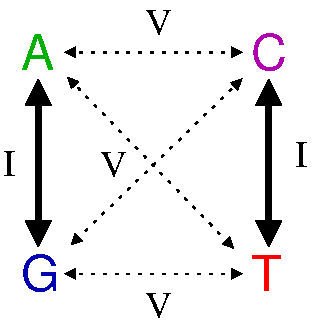
\includegraphics[width=0.9\textwidth]{./graph/IV_figure}
\end{figure}
\end{column}

\end{columns}

for $y \neq x$, $q_{xx} = -\sum_{y \neq x} q_{xy}$ where
$x, y \in \{\colorA, \colorG, \colorC, \colorT \color{black} \}$.

\vspace{0.3cm}
{\scriptsize
$
\bordermatrix{
~       &  \colorA                   & \colorG                & \colorC                & \colorT                \cr
\colorA & 1-\kappa\piG - \piC - \piT & \kappa\piG             & \piC                   & \piT                   \cr
\colorG & \kappa\piA                 & 1-\kappa\piA-\piC-\piT & \piC                   & \piT                   \cr
\colorC & \piA                       & \piG                   & 1-\piA-\piG-\kappa\piT & \kappa\piT             \cr
\colorT & \piA                       & \piG                   & \kappa\piC             & 1-\piA-\piG-\kappa\piC \cr
}
$
}

\vspace{0.2cm}
\begin{center}
\fbox{
CTMC: if $\vect{Q}_{x,y} = \vect{UDU}^{-1}
\Rightarrow
\vect{P}_{x,y}(t)
= e^{\vect{Q}_{x,y}t}
= \vect{U} e^{\vect{D}t} \vect{U}^{-1}
$
}
\end{center}

\end{frame}

%-----------------------------------------------------------------------------

\subsection{Mixture Transition Probability}

\begin{frame}{Transition Probability}

\vspace{-0.3cm}
\begin{figure}
\centering
  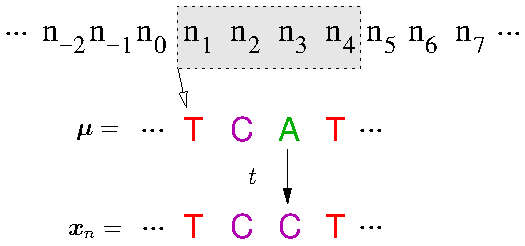
\includegraphics[width=2.0in]{./graph/nucle_figure}
\end{figure}

\vspace{-0.4cm}
\begin{itemize}
\item
$\vect{x}_n = (x_{n1}, \ldots, x_{nL}) \in \mathcal{S}^L$ where
$x_{nl} \in \mathcal{S} = \{\colorA, \colorG, \colorC, \colorT \color{black} \}$. \\

\begin{itemize}
\item Assume mutations among sites are independent.

\item Assume $\vect{x}_n$ evolves from a population center
      $\vect{\mu} = (\mu_1,\ldots, \mu_L) \in \mathcal{S}^L$.

\item Assume an substitution model, $\vect{Q}_{x,y}$.

\item Assume evolving time $t$ between $\vect{\mu}$ and $\vect{x}_n$.
\end{itemize}
Transition probability:
$
p_{\vect{\mu},\vect{x}_n}(t)
= \prod_{l = 1}^L P_{\mu_{kl}, x_{nl}}(t).
$

%\vspace{0.2cm}
\item
Distribution of mutation process:
\begin{center}
\fbox{
$
\phi(\vect{x}_n | \vect{\mu}, \vect{Q}, t) =
p_{\vect{\mu}, \vect{x}_n}(t).
$
}
\end{center}

\end{itemize}

\end{frame}

%-----------------------------------------------------------------------------

\begin{frame}{Mixture Transition Probability}

Mixture Transition Probability:
\begin{itemize}

\item
Mixture proportion:
$\vect{\eta} = (\eta_1, \ldots, \eta_K)$, $\eta_k > 0$, and $\sum_{k = 1}^K \eta_k = 1$.

\item
Dominant sequence (Center):
%$\vect{\mu}_k$.
$\vect{\mu}_k = (\mu_{k1}, \ldots, \mu_{kL}) \in \mathcal{S}^L$ where
$\mu_{kl} \in \mathcal{S}$.

\item
CTMC model (Dispersion): $\vect{Q}_k$ and $t_k$.
\end{itemize}

\vspace{0.2cm}
Possible CTMC models:
\begin{itemize}
\item
EE: $\vect{Q}_1 = \vect{Q}_2 = \cdots = \vect{Q}_K$
          and $t_1 = t_2 = \cdots = t_K$.
\item
EV: $\vect{Q}_1 = \vect{Q}_2 = \cdots = \vect{Q}_K$
          and $t_1 \neq t_2 \neq \cdots \neq t_K$.
\item
VE: $\vect{Q}_1 \neq \vect{Q}_2 \neq \cdots \neq \vect{Q}_K$
          and $t_1 = t_2 = \cdots = t_K$.
\item
VV: $\vect{Q}_1 \neq \vect{Q}_2 \neq \cdots \neq \vect{Q}_K$
          and $t_1 \neq t_2 \neq \cdots \neq t_K$.
\end{itemize}

\end{frame}

%-----------------------------------------------------------------------------

\begin{frame}{Examples of CTMC models}

\vspace{-0.5cm}
\begin{columns}

\begin{column}{0.5\textwidth}
  \begin{figure}
  \begin{center}
  EE\\
    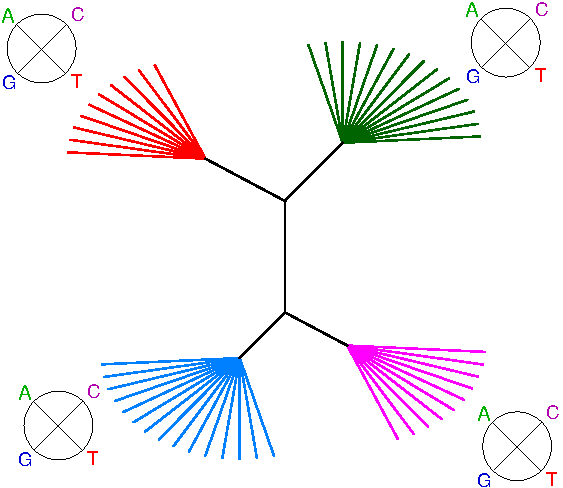
\includegraphics[width=0.75\textwidth]{./graph/tree_EE}
  %\end{center}
  %\end{figure}

  \vspace{0.2cm}
  %\begin{figure}
  %\begin{center}
  VE\\
    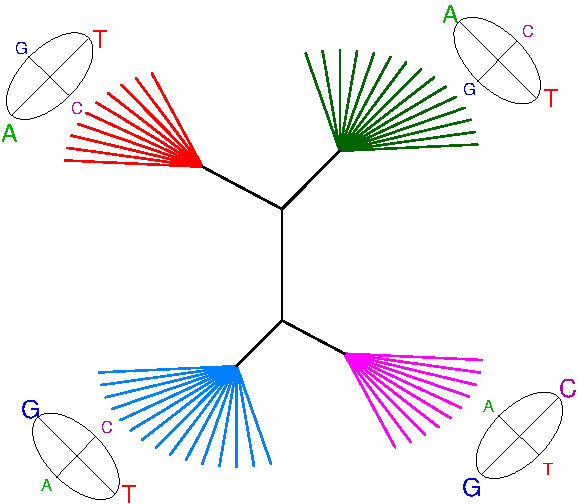
\includegraphics[width=0.75\textwidth]{./graph/tree_VE}
  \end{center}
  \end{figure}
\end{column}

\begin{column}{0.5\textwidth}
  \begin{figure}
  \begin{center}
  EV\\
    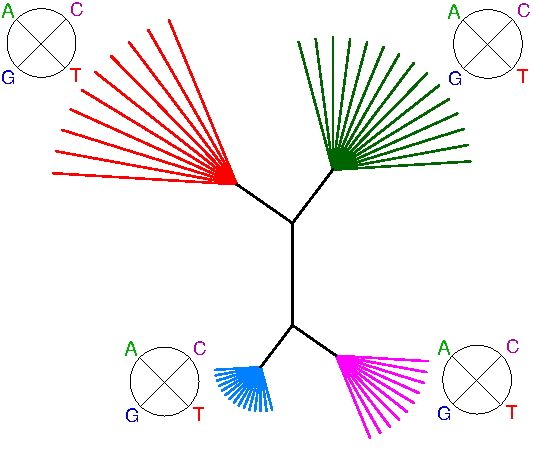
\includegraphics[width=0.75\textwidth]{./graph/tree_EV}
  %\end{center}
  %\end{figure}

  \vspace{0.2cm}
  %\begin{figure}
  %\begin{center}
  VV\\
    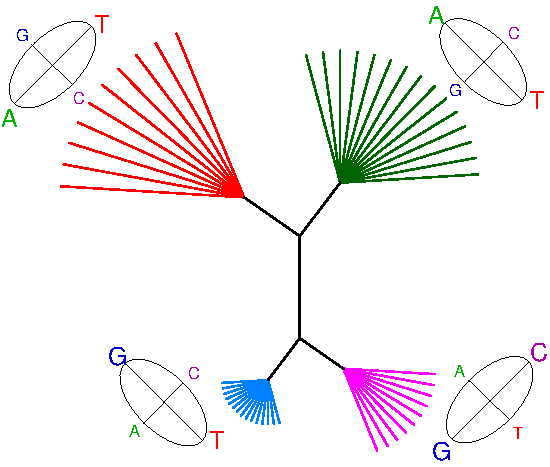
\includegraphics[width=0.75\textwidth]{./graph/tree_VV}
  \end{center}
  \end{figure}
\end{column}

\end{columns}

\end{frame}

%-----------------------------------------------------------------------------

\subsection{EM Algorithm}

\begin{frame}{EM Algorithm for Mixture Model}

\begin{itemize}
\item Log likelihood:
let $\vect{\Theta} = \{\vect{\eta}, \vect{\mu}, \vect{Q}, t\}$,
\begin{center}
$
\log L(\vect{\Theta} | \vect{x})
 = \sum_{n=1}^N \log \left[
   \sum_{k = 1}^K \eta_k \phi_k(\vect{x}_n| \vect{\mu}_k, \vect{Q}_k, t_k)
   \right ].
$
\end{center}


\item Augment data for missing information:
\begin{center}
$Z_{nk} = I(n \in \mathcal{G}_k)$
for $n = 1, \ldots, N$ and $k = 1, \ldots, K$.
\end{center}


\item Log complete-data likelihood:
\end{itemize}
\begin{center}
$
\log L_c(\vect{\Theta}, \vect{Z} | \vect{x}) =
\sum_{n = 1}^N
\sum_{k=1}^K
Z_{nk}
\left[ \log \eta_k + \log \phi_k(\vect{x}_n| \vect{\mu}_k, \vect{Q}_k, t_k)
\right].
$
\end{center}

\begin{itemize}
\item EM algorithm:  (Dempster et.al. 1977)

\begin{enumerate}
\item E-step:
$
Q(\vect{\Theta} | \vect{x}) =
\E_{\vect{Z}} [\log L_c(\vect{\Theta},\vect{Z} | \vect{x})].
$

\item M-step:
$
\max_{\vect{\Theta}} Q(\vect{\Theta} | \vect{x}).
$

\item Iterate E- and M-steps until convergence which yields
$$
\hat{\vect{\Theta}} = \argmax_{\vect{\Theta}} \log L(\vect{\Theta} | \vect{x}).
$$
\end{enumerate}

\end{itemize}
\end{frame}

%-----------------------------------------------------------------------------

\begin{frame}{EM Algorithm for Phyloclustering with EE Model}

\begin{itemize}
\item
E-step:
\begin{center}
$
z_{nk}^{(s)} =
\E_{\vect{Z}} [ Z_{nk} | \vect{x}, \vect{\Theta}^{(s-1)} ] =
\frac{
\eta_k^{(s-1)}
\phi_k(\vect{x}_n|
\vect{\mu}_k^{(s-1)}, \vect{Q}^{(s-1)}, t^{(s-1)})
}{
\phi(\vect{x}_n|
\vect{\mu}^{(s-1)}, \vect{Q}^{(s-1)}, t^{(s-1)})
}$
\end{center}
where $n = 1, \ldots, N$ and $k = 1, \ldots, K$.

\item
M-step:

\begin{itemize}
\item
$\eta_k^{(s)} = \sum_{n=1}^N z_{nk}^{(s)} / N$.

\item
$\vect{\mu}_k^{(s)}(\vect{Q}, \vect{t})$ obtained by
comparing transition probabilities,

\vspace{-0.2cm}
\begin{columns}
\begin{column}{\textwidth}
$$
\begin{array}{rcl}
\mu_{kl}^{(s)}(\vect{Q}, t)
 &=& \dargmax{\mu \in \mathcal{S}}
     \sum_{n = 1}^N z_{nk}^{(s)} \log \phi_k(x_{nl}| \mu(\vect{Q}, t), \vect{Q}, t) \\
 &=& \dargmax{\mu \in \mathcal{S}}

\sum_{a \in \mathcal{S}}
\left[
\left(
\sum_{n \ni x_{nl} = a} z_{nk}^{(s)}
\right)
N_{\{x_l = a\}} \log p_{\mu, s}(t)
\right].

\end{array}
$$
\end{column}
\end{columns}
\vspace{0.1cm}

\item
$\vect{Q}^{(s)}$ and $t^{(s)}$ obtained numerically to maximize profile likelihood.

\end{itemize}

\end{itemize}

\end{frame}

%-----------------------------------------------------------------------------

\begin{frame}{Challenges of EM Algorithm}

\begin{enumerate}
\item Improve slow confergence of EM algorithm:
\begin{itemize}
\item ECM (Meng \& Rubin (1993)).
\item AECM (Meng \& van Dyk (1997)).
\item APECM (Chen \& Maitra (2011)).
\end{itemize}

\item Initialization schemes to improve convergent results:

-- Method:
\begin{itemize}
\item Neighbor joining tree (Saitou \& Nei (1987))
\item Partition Around Medoids (PAM) (Kaufman \& Rousseeuw (1990))
\item K-Medoids (Theodoridis \& Koutroumbas (2006))
\item Manually
\end{itemize}

-- Procedure:
\begin{itemize}
\item em-EM (Biernacki, Celeux, \& Govaert (2003))
\item Rand-EM (Maitra (2007))
\item Exhausted EM
\end{itemize}

\end{enumerate}

\end{frame}

%-----------------------------------------------------------------------------

\section{Simulation Study}

\begin{frame}{Simulation Study I}

\vspace{-0.1cm}
\begin{center}
\begin{figure}
  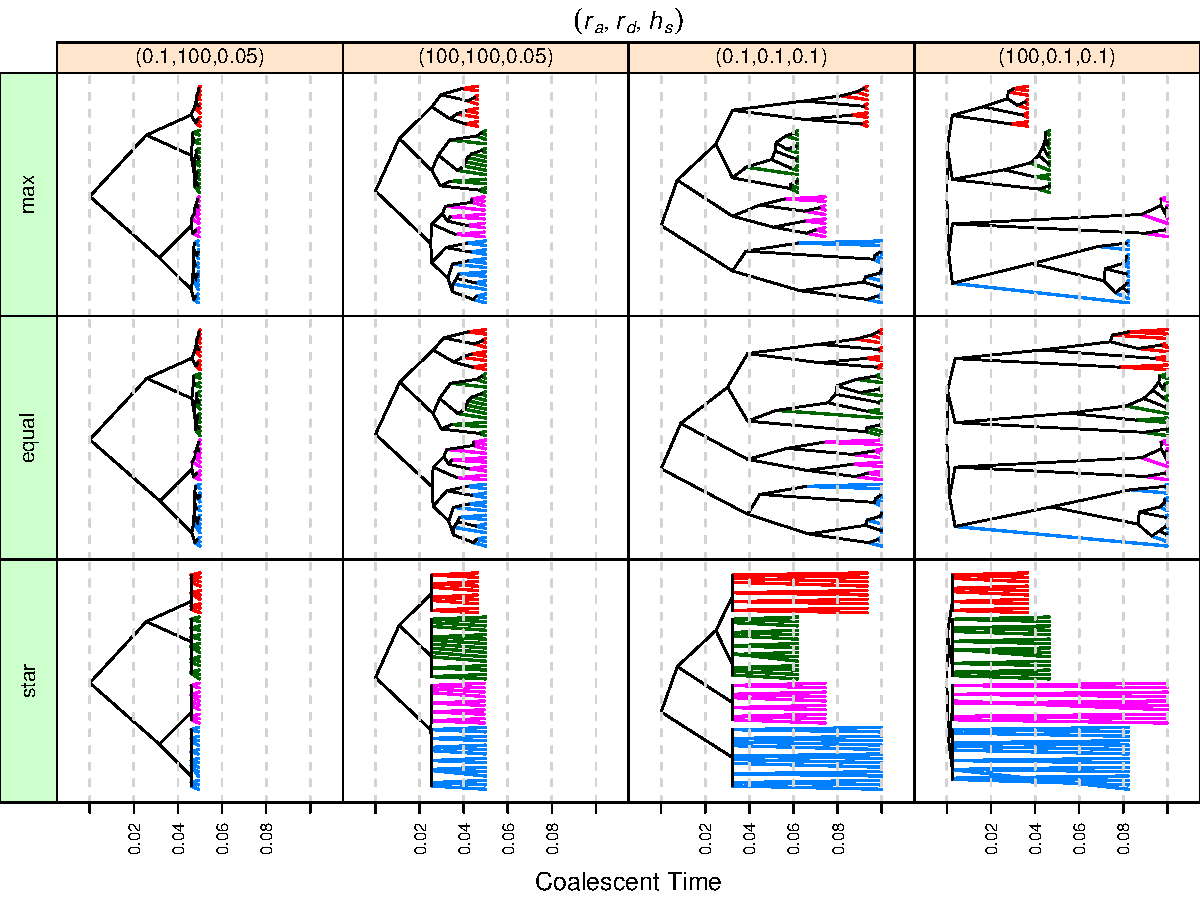
\includegraphics[width=\textwidth]{./graph/ex_tree_a_sub}
  \\
  \vspace{-0.2cm}
  {\tiny
  $r_a$: growth rate of ancestor tree,
  $r_d$: growth rate of descendent tree,
  $h_s$: total height.}
\end{figure}
\end{center}

\end{frame}

%-----------------------------------------------------------------------------

\begin{frame}{Results of Simulation Study I}

\vspace{-0.8cm}
\begin{columns}

\hspace{-1.2cm}
\begin{column}{\textwidth}
\begin{figure}
  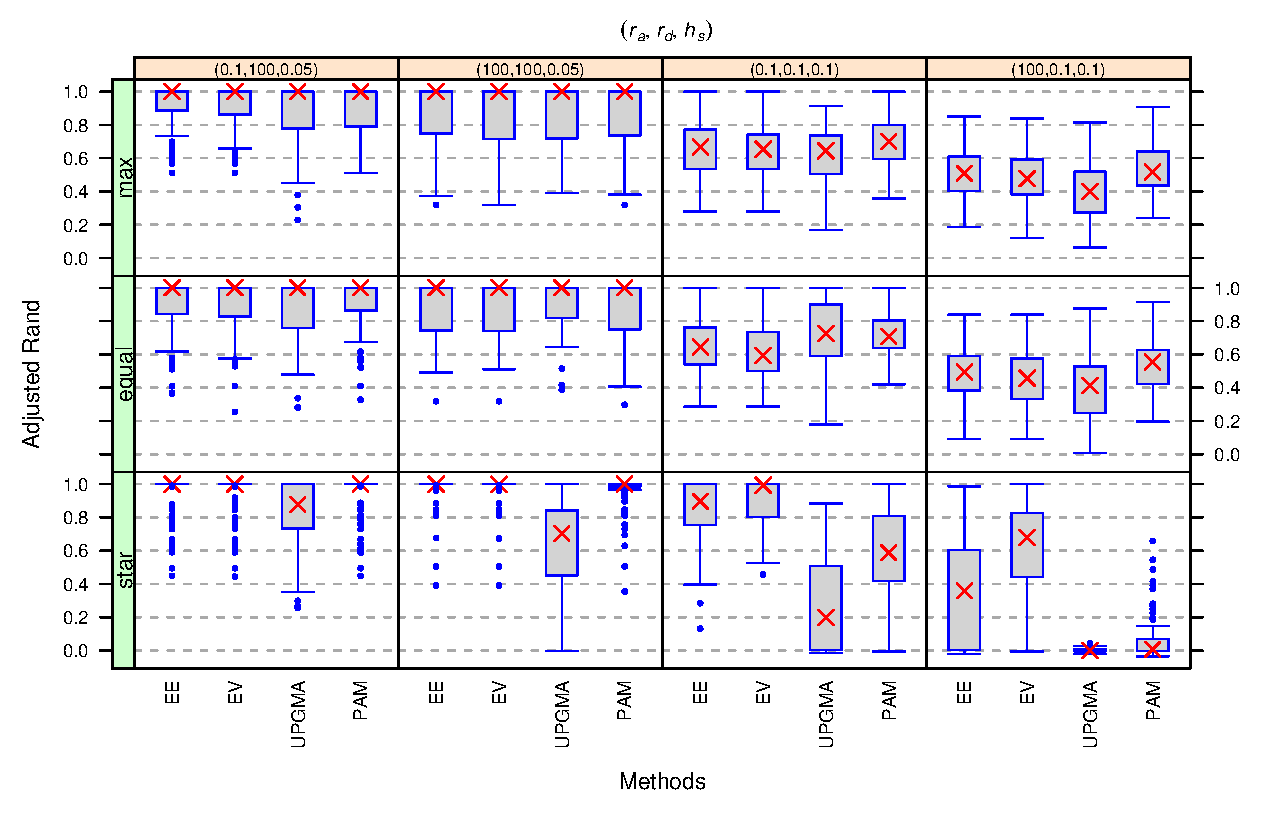
\includegraphics[width=4.7in]{./graph/simulation_a_sub}
  \\
  \vspace{-0.2cm}
  {\tiny Results of EE (phyclust), EV (phyclust), UPGMA, and PAM.}
\end{figure}
\end{column}

\end{columns}

\end{frame}

%-----------------------------------------------------------------------------

\begin{frame}{Simulation Study II and Results}

\vspace{-0.1cm}
\begin{center}
\begin{figure}
  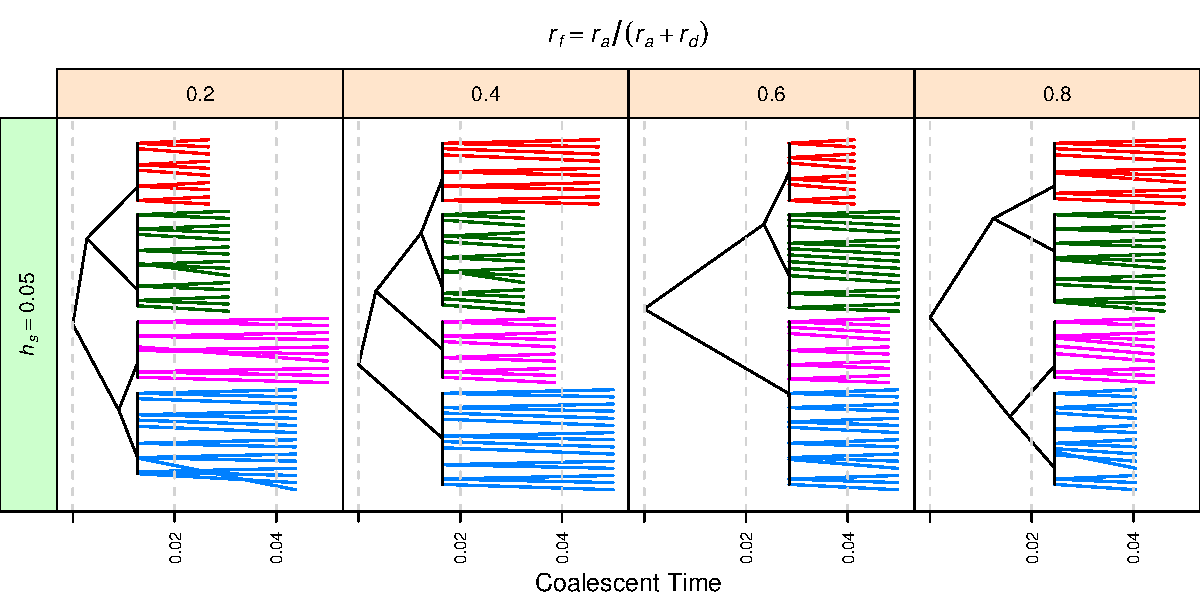
\includegraphics[width=3.5in]{./graph/ex_tree_b_sub}
\end{figure}

\vspace{-1.0cm}
\begin{columns}

\hspace{-0.7cm}
\begin{column}{0.5\textwidth}
\begin{figure}
  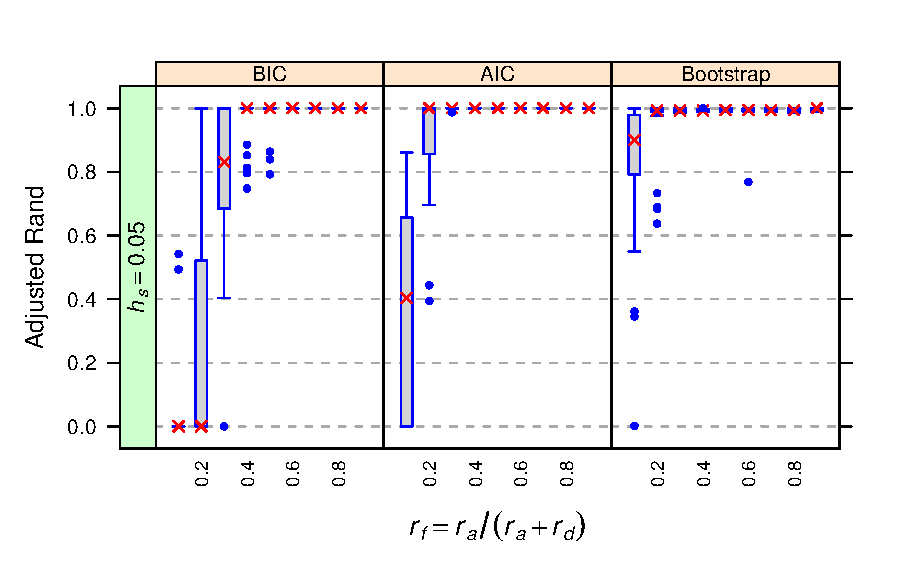
\includegraphics[width=2.5in]{./graph/simulation_b_1_sub}
\end{figure}
\end{column}

\hspace{-0.3cm}
\begin{column}{0.5\textwidth}
\begin{figure}
  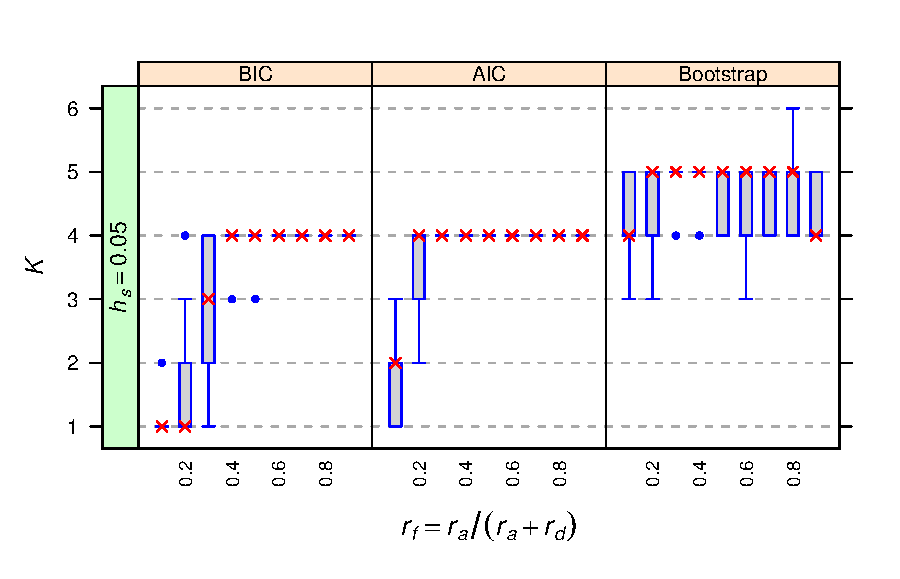
\includegraphics[width=2.5in]{./graph/simulation_b_2_sub}
\end{figure}
\end{column}

\end{columns}
\end{center}

\end{frame}

%-----------------------------------------------------------------------------

\section{Data Analysis}

\subsection{EIAV Result}

\begin{frame}{EIA Disease Progress}

\vspace{-1.5cm}
\begin{center}
\hspace{-1.6cm}
\begin{figure}
  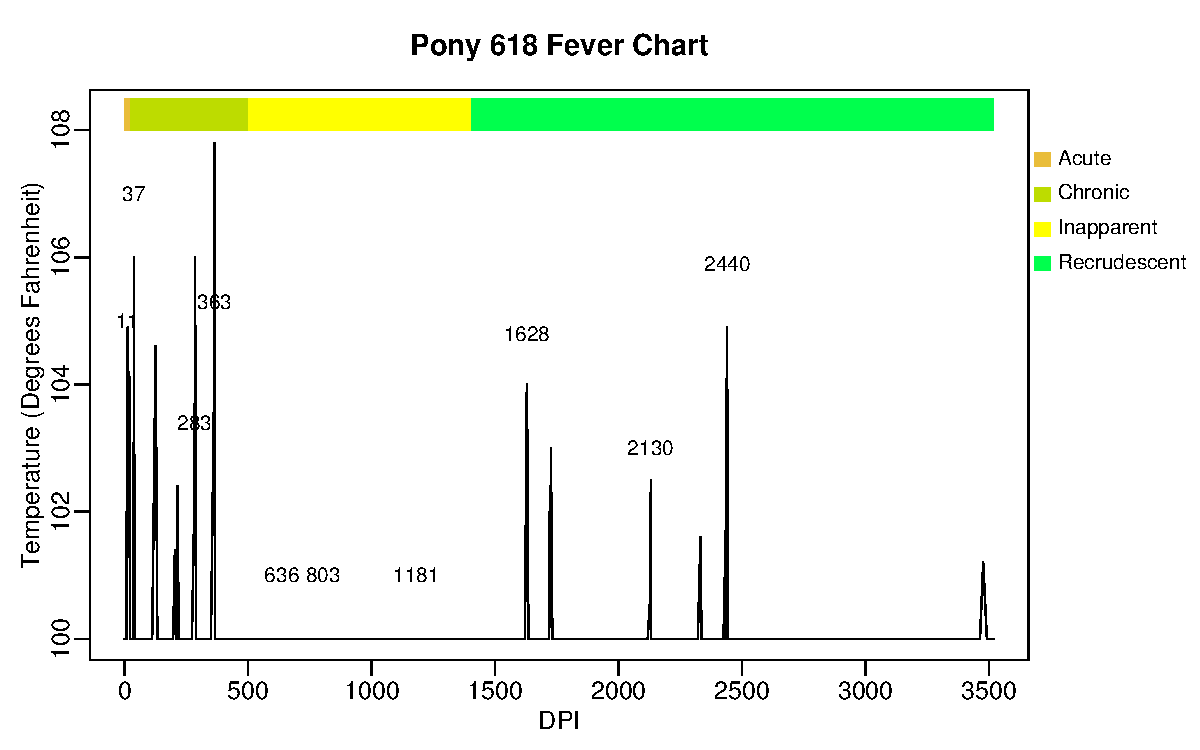
\includegraphics[width=4.5in]{./graph/fever_cycle}
  \\
  \vspace{-0.2cm}
  {\tiny Cierra Pairett (2011), ''Longitudinal analysis of genetic and antigenic
  variation in EIAV env'', Iowa State University.}
\end{figure}
\end{center}

\end{frame}

%-----------------------------------------------------------------------------

\begin{frame}{EIAV Phyloclustering Results}

\vspace{-1.0cm}
\begin{columns}

\hspace{-1.0cm}
\begin{column}{\textwidth}
\begin{figure}
  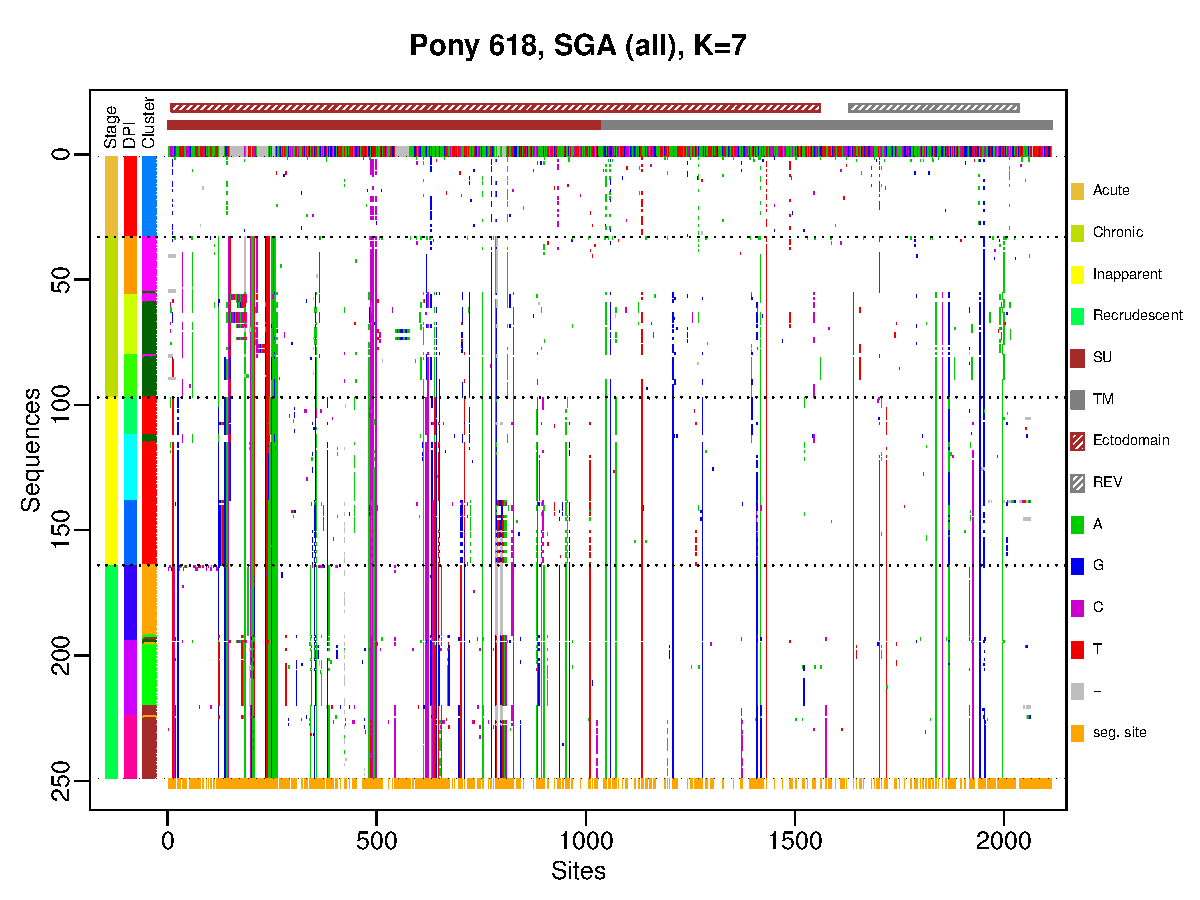
\includegraphics[width=4.6in]{./graph/SGA_sort_all_K=7}
\end{figure}
\end{column}

\end{columns}

\end{frame}

%-----------------------------------------------------------------------------

\begin{frame}{EIAV ID50 Result}

\vspace{-0.2cm}
\begin{figure}
  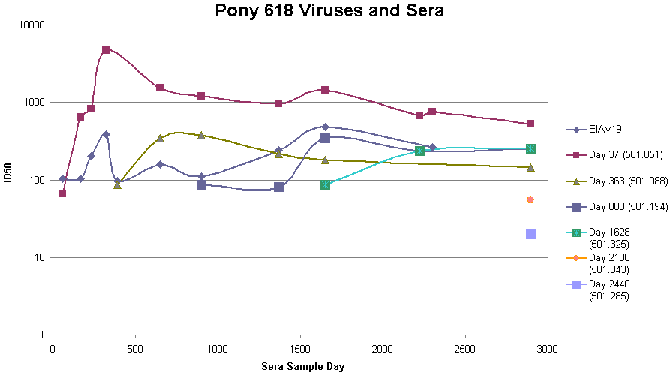
\includegraphics[width=4.5in]{./graph/cierra}
  \\
  \vspace{-0.1cm}
  {\tiny Cierra Pairett (2011), ''Longitudinal analysis of genetic and antigenic
  variation in EIAV env'', Iowa State University.}
\end{figure}

\end{frame}

%-----------------------------------------------------------------------------

\begin{frame}{EIAV Tree}

\begin{center}
\vspace{-0.5cm}
\begin{figure}
\hspace{-1.0cm}
  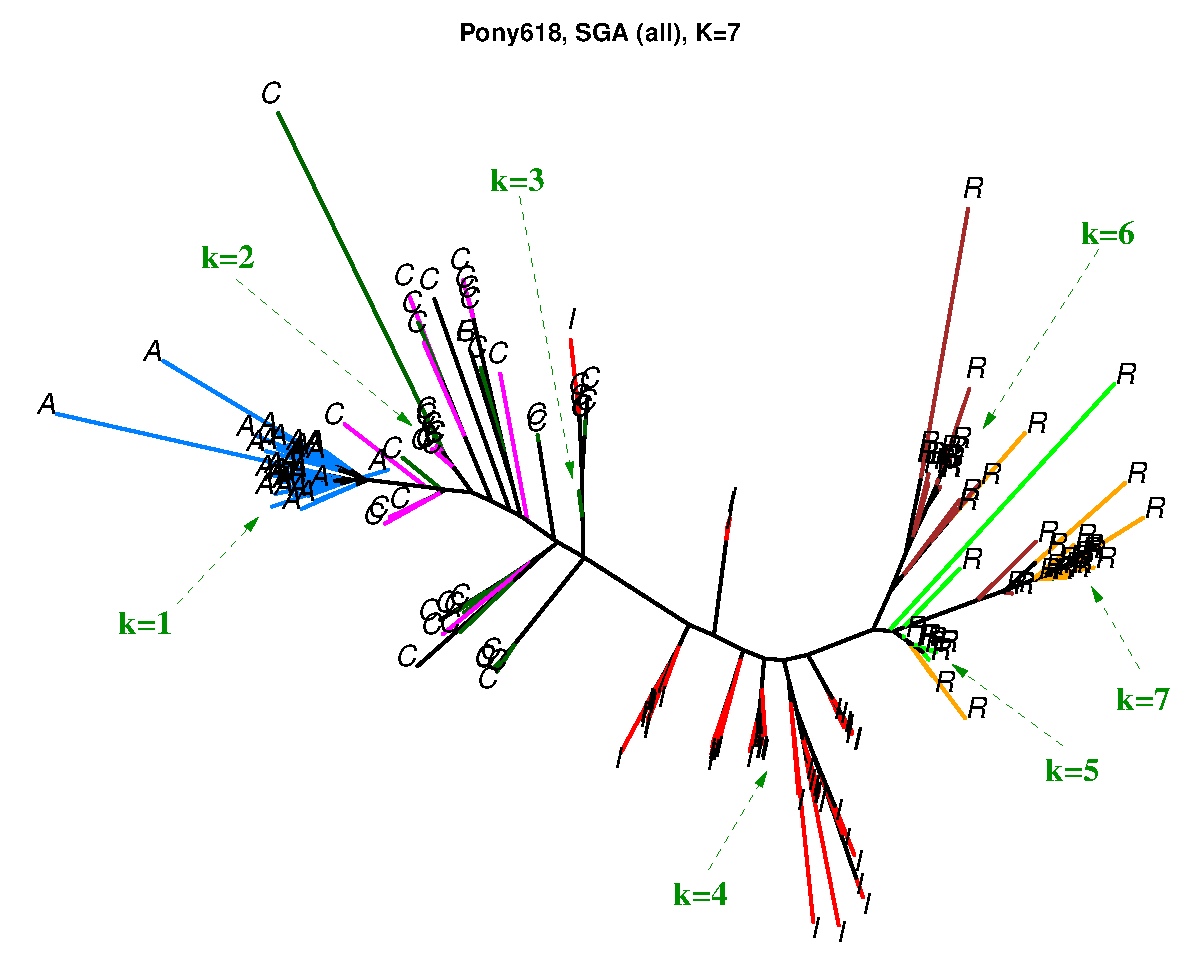
\includegraphics[width=4.2in]{./graph/SGA_tree_K=7}
  \\
  \vspace{-0.5cm}
  {\tiny A: Acute, C: Chronic, I: Inapparent, R: Recrudescent.}
\end{figure}
\end{center}

\end{frame}

%-----------------------------------------------------------------------------

\section{Summary}

\begin{frame}{Summary}

\begin{itemize}
\item {\tt phyclust}: an \R package for Phylogenetic Clustering
      ({\tt https://cran.r-project.org/package=phyclust}).
\item Identify number of clusters.
\item Initialization problem for EM algorithm.
\item Potential extensions:
\begin{itemize}
\item Reduce number of parameters (Hierarchical model for center sequences.)
\item Dependent structure along sites (Hidden Markov model.)
\end{itemize}
\end{itemize}

\end{frame}

%-----------------------------------------------------------------------------

\begin{frame}{Acknowledgement}

\begin{itemize}
\item Dr. Karin Dorman
\item Dr. Ranjan Maitra
\item Dr. Susan Carpenter
\item Cierra Pairett
\end{itemize}

\vspace{2.5cm}
\Huge
\centering
\color{dgreen}
{\it Thank you!}

\end{frame}


\end{document}

